% Modelo de Trabalho Acadêmico da UNESP de Guaratinguetá v-1.0
% Copyright 2017 by Eduardo Rohde Eras
%
% This program is free software: you can redistribute it and/or modify
% it under the terms of the GNU General Public License as published by
% the Free Software Foundation, either version 3 of the License, or
% (at your option) any later version.
%
% This program is distributed in the hope that it will be useful,
% but WITHOUT ANY WARRANTY; without even the implied warranty of
% MERCHANTABILITY or FITNESS FOR A PARTICULAR PURPOSE.  See the
% GNU General Public License for more details.
%
% You should have received a copy of the GNU General Public License
% along with this program.  If not, see <http://www.gnu.org/licenses/>.

%----------------------------------------------------------------------------------------%
% C L A S S E   D O   D O C U M E N T O
%----------------------------------------------------------------------------------------%

\documentclass[
  %----------------------------------------------------------------------------------------%
  %Opções da classe 'memoir'
  %----------------------------------------------------------------------------------------%
  12pt,		% Tamanho da Fonte.
  a4paper,	% Tamanho da página.
  openright,% Capítulos começam em páginas ímpares (insere uma página vazia se necessário).
  oneside,	% Para impressão em frente e verso utilizar twoside.
  %----------------------------------------------------------------------------------------%
  %Opções da classe 'abntex2'
  %----------------------------------------------------------------------------------------%
  chapter=TITLE,		%Títulos de capítulos convertidos em letras maiúsculas.
  section=TITLE,		%Títulos de seções convertidos em letras maiúsculas.
  %----------------------------------------------------------------------------------------%
  %Opções da classe 'babel'
  %----------------------------------------------------------------------------------------%
  english,	%Idioma adicional para hifenização.
  french,	%Idioma adicional para hifenização.
  spanish,	%Idioma adicional para hifenização.
  brazil
  %----------------------------------------------------------------------------------------%
]{abntex2}

%----------------------------------------------------------------------------------------%
% P A C O T E S
%
% Insira aqui os pacotes que for utilizar em seu documento. Para saber quais pacotes o
% template já está utilizando, confira o arquivo "pacoteBasico.sty".
%----------------------------------------------------------------------------------------%
    
    \usepackage{pacoteBasico}   %Pacote Básico de formatação no padrão da UNESP/FEG
    \usepackage{color}		    %Controle das cores.
    \usepackage{graphicx}	    %Inclusão de gráficos.
    \usepackage{lipsum}		    %Para geração de 'Dummy Text'.
    \usepackage{lastpage}       % usado por abntex2-fichacatalografica.tex
    %packages para geração: tabelas longas (longtable), com melhor layout (booktabs), multiplas linhas (multirow), folha em modo paisagem para tabelas largas (lscape)
    \usepackage{longtable, booktabs, multirow, lscape}  
    %forçar o posicionamento dos ambientes https://en.wikibooks.org/wiki/LaTeX/Floats,_Figures_and_Captions
    \usepackage{float}

    
%----------------------------------------------------------------------------------------%
% I N F O R M A Ç Õ E S   B Á S I C A S   S O B R E   O   T R A B A L H O
%
% Defina aqui as informações pertinentes ao trabalho.
%----------------------------------------------------------------------------------------%

    %----------------------------------------------------------------------------------------%
    % D A D O S   P E S S O A I S
    %----------------------------------------------------------------------------------------%
    
    %Nome completo do autor do presente Trabalho de Graduação:
    \newcommand{\nomeDoAutor}{
    Nome Completo do Autor
    }
    
    %Nome do curso em que o autor está se graduando:
    \newcommand{\nomeDoCurso}{
    Nome do Curso
    }
    
    %----------------------------------------------------------------------------------------%
    % D A D O S   S O B R E   O   T R A B A L H O
    %----------------------------------------------------------------------------------------%
    
    %Título do presente trabalho:
    \newcommand{\tituloDoTrabalho}{Título do trabalho somente com a primeira palavra em maiúsculo}
    
    %Subtítulo do presente trabalho, se houver:
    \newcommand{\subtituloDoTrabalho}{subtítulo do trabalho, se houver, todo em minúsculo}
    
    %Mês da entrega do trabalho
    \newcommand{\mesDeEntrega}{Fevereiro}
    
    %Ano da entrega do trabalho
    \newcommand{\anoDeEntrega}{2019}
    
    %----------------------------------------------------------------------------------------%
    % D A D O S   D O S   O R I E N T A D O R E S,   B A N C A   E   C O O R D E N A D O R
    %----------------------------------------------------------------------------------------%
    
    %Nome do orientador do presente trabalho:
    \newcommand{\nomeDoOrientador}{
    Nome Completo do Orientador
    }
    
    %Título do orientador:
    \newcommand{\tituloDoOrientador}{
    Profº Dr.
    }
    
    %Nome do coorientador do presente trabalho:
    \newcommand{\NomeDoCoorientador}{
    Nome Completo do Coorientador
    }
    
    %Título do coorientador:
    \newcommand{\tituloDoCoorientador}{
    Profº Dr.
    }
    
    %Nome do Coordenador do Curso:
    \newcommand{\nomeDoCoordenador}{
    Nome Completo do Coordenador
    }
    
    %Título do coordenador do Curso:
    \newcommand{\tituloDoCoordenador}{
    Profº Dr.
    }
    
    %Nome do Membro Interno da Banca:
    \newcommand{\nomeDoMembroInterno}{
    Nome Completo do Membro Interno
    }
    
    %Título do Membro Interno da Banca:
    \newcommand{\tituloDoMembroInterno}{
    Profº Dr.
    }
    
    %Nome do membro Externo da banca:
    \newcommand{\nomeDoMembroExterno}{
    Nome Completo do Membro Externo
    }
    
    %Título do Membro Externo da Banca:
    \newcommand{\tituloDoMembroExterno}{
    Profº Dr.
    }
    
    %----------------------------------------------------------------------------------------%
    % D A D O S   D A   I N S T I T U I Ç Ã O
    %----------------------------------------------------------------------------------------%
    
    %Nome da Universidade
    \newcommand{\nomeDaUniversidade}{
    Universidade Estadual Paulista "Júlio de Mesquita Filho"
    }
    
    %Nome da Cidade
    \newcommand{\nomeDaCidade}{
    Guaratinguetá
    }

%----------------------------------------------------------------------------------------%
% I N Í C I O   D O   D O C U M E N T O - P R É   T E X T U A L
%----------------------------------------------------------------------------------------%
\begin{document}
    
    \imprimircapa
    \imprimirfolhaderosto
    
    %------------------------------------------------------------------------------------%
    % F I C H A   CATALOGRÁFICA
    %
    % OBRIGATÓRIO. Esta ficha é gerada pela Biblioteca depois de efetuar as correções  
    % sugeridas pela banca da defesa do trabalho. Aqui, foi adicionado o exemplo encontrado
    % na documentação 'A classe abntex2' (p. 23). Recomenda-se, contudo, adicionar o arquivo
    % enviado pela biblioteca no formato em pdf. Para isso, basta excluir tudo, a adicionar
    % \includepdf{fichacatalografica.pdf} através do pacote pdfpages
    %------------------------------------------------------------------------------------%
    \begin{fichacatalografica}
     %\sffamily
        \vspace*{15cm} % Posição vertical
        \hrule % Linha horizontal
        \begin{center} % Minipage Centralizado
        \begin{minipage}[c]{12.5cm} % Largura
        %\nomeDoAutor
        %\hspace{0.5cm} \tituloDoTrabalho: \subtituloDoTrabalho / \nomeDoAutor. --
        %\nomeDaCidade, \mesDeEntrega \anoDeEntrega-
        %\hspace{0.5cm} \pageref{LastPage} p. : il.(alguma color.); 30 cm.\\
        %\hspace{0.5cm} \tituloDoOrientador \nomeDoOrientador\\
        %\hspace{0.5cm}
        %\parbox[t]{\textwidth}{\imprimirtipotrabalho~--~\nomeDaUniversidade,
        %\mesDeEntrega \anoDeEntrega.}\\
        %\hspace{0.5cm}
        %1. Palavra-chave1.
        %2. Palavra-chave2.
        %I. Orientador.
        %II. Universidade xxx.
        %III. Faculdade de xxx.
        %IV. Título\\
        %\hspace{8.75cm} CDU 02:141:005.7\\
        A confecção da ficha catalográfica é realizada exclusivamente pelo Serviço Técnico de Biblioteca e Documentação. Para solicitá-la, use o formulário eletrônico disponível em: \url{http://www2.feg.unesp.br/#!/biblioteca/trabalho-conclusao-de-curso/}.
        \\
        \\
    
         A adição da ficha catalográfica no \LaTeX é ainda um problema em aberto (issue $\#$01 \url{https://github.com/luisfelipebarbosa/feg-latex/issues/1})
        
        \end{minipage}
        \end{center}
        \hrule
    \end{fichacatalografica}
    

    
    
    %------------------------------------------------------------------------------------%
    % F O L H A   D E   A P R O V A Ç Ã O
    %
    % OBRIGATÓRIO. Este é o modelo de folha de aprovação que deve ser digitalizada após as
    % assinaturas da banca. Utilize um software de edição de PDF para substituição posterior
    % dessa folha. Se possível, utilize um recurso de assinatura digital fornecido pela
    % ferramenta de edição de PDF, evitando assim a digitalização da folha toda.
    %------------------------------------------------------------------------------------%
    \begin{folhadeaprovacao}
        \begin{center}
        
        {\sffamily
            \bfseries{
                \Large{
                    UNIVERSIDADE ESTADUAL PAULISTA\par
                    "JÚLIO DE MESQUITA FILHO"\par
                }
            }
            CAMPUS DE GUARATINGUETÁ
        }
        
        \vspace*{3cm}
                
        \normalsize{\textbf{\MakeUppercase\nomeDoAutor}}
        
        \vspace*{1cm}
        
       % {\setstretch{1.0}
        \begin{framed}
            ESTE TRABALHO DE GRADUAÇÃO FOI JULGADO ADEQUADO COMO PARTE DO REQUISITO PARA A OBTENÇÃO DO DIPLOMA DE \textbf{"GRADUANDO EM {\MakeUppercase\nomeDoCurso}"}
            \par
            \vspace*{1cm}
            APROVADO EM SUA FORMA FINAL PELO CONSELHO DE CURSO DE GRADUAÇÃO EM {\MakeUppercase\nomeDoCurso}
            \par
            \vspace*{1cm}
            \begin{flushright}
            \tituloDoCoordenador {\MakeUppercase\nomeDoCoordenador}
            \par
            Coordenador
            \end{flushright}
       \end{framed}
      % }
       
       \begin{flushleft}
            \textbf{BANCA EXAMINADORA:}
       \end{flushleft}
       
       \assinatura{\small \tituloDoOrientador \nomeDoOrientador \par Orientador/UNESP-FEG}
       \assinatura{\small \tituloDoMembroInterno \nomeDoMembroInterno \par UNESP-FEG}
       \assinatura{\small \tituloDoMembroExterno \nomeDoMembroExterno \par Membro Externo}
       
       \vfill
       \mesDeEntrega, \anoDeEntrega
        
        \end{center}
    \end{folhadeaprovacao}

    
    
    

    
    %------------------------------------------------------------------------------------%
    % D A D O S   C U R R I C U L A R E S
    % 
    % OBRIGATÓRIO PARA PÓS-GRADUAÇÃO.
    % Inserir a data inicial e final de cada formação acadêmica. Para os alunos que não
    % precisarem de uma folha de dados curriculares em seu trabalho, basta apagar todo 
    % o código dessa seção.
    %------------------------------------------------------------------------------------%
    
    \begin{center}
        \normalsize{\textbf{\MakeUppercase{Dados Curriculares}}} \par
        \vspace*{1cm}
        \normalsize{\textbf{\MakeUppercase\nomeDoAutor}} \par
        \vspace*{1cm}
        
        \begin{tabular}{ l p{7cm} }
            \textbf{\MakeUppercase{Nascimento}} & Data - Cidade / Sigla do Estado \\
            \\
            \textbf{\MakeUppercase{Filiação}} & Nome completo do Pai \\
            & Nome completo da Mãe \\
            \\
            \textbf{\MakeUppercase{Ano Inicial / Ano Final}} & Formação acadêmica ou Complementar (nome do curso e titulação) \\
            & Instituição de Ensino \\
            \\
            \textbf{\MakeUppercase{Ano Inicial / Ano Final}} & Formação acadêmica ou Complementar (nome do curso e titulação) \\
            & Instituição de Ensino \\
            \\
            \textbf{\MakeUppercase{Ano Inicial / Ano Final}} & Formação acadêmica ou Complementar (nome do curso e titulação) \\
            & Instituição de Ensino \\
        \end{tabular}
    \end{center}
    \newpage
    
    %------------------------------------------------------------------------------------%
    % D E D I C A T Ó R I A
    %
    % OPCIONAL. Se não for utilizar uma dedicatória, basta apagar todo o código dessa seção.
    %------------------------------------------------------------------------------------%
    
    \begin{dedicatoria}
        \vspace*{\fill}
        \begin{flushright}
            Sua dedicatoria deve ser digitada aqui.
        \end{flushright}
        \vspace*{1cm}
    \end{dedicatoria}

    %------------------------------------------------------------------------------------%
    % A G R A D E C I M E N T O S
    %
    % OPCIONAL. Citar as pessoas, instituição, agência de fomento, entre outros que contribuíram
    % de maneira relevante à elaboração do trabalho e na vida acadêmica.
    % Se não for utilizar os agradecimentos, basta apagar todo o código dessa seção.
    %------------------------------------------------------------------------------------%
    \begin{agradecimentos}
    
        Esse é um espaço reservado para os agradecimentos. Uma nota de rodapé\footnote{Essa é uma nota de rodapé} pode ser inserida desta forma para indicar alguma URL\footnote{\url{http:\\www.url.com.br}} que referencia o alvo de seu agradecimento.
    
    \end{agradecimentos}
    
    %------------------------------------------------------------------------------------%
    % F O M E N T O
    %
    % OBRIGATÓRIO PARA ALUNO BOLSISTA. Esta página contém informações sobre o financiamento
    % recebido para o desenvolvimento da tese/dissertação. Utilize o(s) nome(s) da(s) 
    % instituição(ões) que forneceu(ram) o auxílio financeiro para seu trabalho. Se não
    % for utilizar o fomento em seu trabalho, basta apagar todo o código dessa seção.
    %------------------------------------------------------------------------------------%
    \vspace*{\fill}
    \begin{flushleft}
        Este trabalho contou com o apoio da(s) seguinte(s) entidade(s):\\
        FAPESP - Fundação de Amparo à Pesquisa do Estado de São Paulo\\
        CAPES - Coordenação de Aperfeiçoamento de Pessoa de Nível Superior\\
        CNPq - Conselho Nacional de Desenvolvimento Científico e Tecnológico\\
        SIGQ - Sigla de Uma Instituição Genérica Qualquer
    \end{flushleft}
    \newpage
    
    %------------------------------------------------------------------------------------%
    % E P Í G R A F E
    %
    % OPCIONAL. Texto em que o autor apresenta uma citação, seguida de indicação de autoria.
    % Se não for utilizar uma epígrafe, basta apagar todo o código dessa seção.
    %------------------------------------------------------------------------------------%
    
    \begin{epigrafe}
        \vspace*{\fill}
    	\begin{flushright}
    		\textit{
        		``Frase, citação, epígrafe.``\\
        		(Autor)
    		}
    	\end{flushright}
    \end{epigrafe}
    
    %------------------------------------------------------------------------------------%
    % R E S U M O   N O   I D I O M A   D O   T E X T O
    %
    % OBRIGATÓRIO. Deve ser redigido em um só parágrafo contendo de 150 a 500 palavras e 
    % ressaltar: objetivo, método, resultados e as principais conclusões.
    % Após o resumo, são listadas palavras-chave relacionadas à temática do trabalho, 
    % separadas entre si por ponto e também finalizadas por ponto.  (NBR 6028, 2003)
    %------------------------------------------------------------------------------------%
    
    \begin{resumo}
    
        \lipsum[1] % Digite seu resumo no lugar deste comando.
        
        \vspace*{0.5cm}
    
        \noindent\textbf{\MakeUppercase{Palavras-Chave: }} Palavra-chave. Palavra-chave.
    
    \end{resumo}
    
    %------------------------------------------------------------------------------------%
    % A B S T R A C T :   R E S U M O   N O   I D I O M A   E S T R A N G E I R O
    %
    % OBRIGATÓRIO. Elaborado com as mesmas características do resumo em língua portuguesa.
    % Se redigido em inglês-ABSTRACT, em castelhano-RESUMEN, em francês-RÉSUMÉ.
    % Após o resumo, são listadas palavras-chave relacionadas à temática do trabalho no 
    % idioma escolhido. Se redigido em inglês - KEYWORDS, em espanhol - PALABRAS CLAVES,
    % em francês - MOTS-CLÉS.
    %------------------------------------------------------------------------------------%
    
    \begin{resumo}[Abstract] % Substitua 'Abstract' pela palavra no idioma desejado, caso precise.
    
        \lipsum[1] % Digite seu abstract no lugar deste comando.
        
        \vspace*{0.5cm}
        
        %Subistitua 'Keywords' pela palavra no idioma desejado, caso precise.
        \noindent\textbf{\MakeUppercase{Keywords: }} Keyword. Keyword. Keyword.
    
    \end{resumo}
    
    %------------------------------------------------------------------------------------%
    % L I S T A   D E   I L U S T R A Ç Õ E S
    %
    % OPCIONAL. Quando necessário recomenda-se a elaboração de lista própria para cada tipo
    % de ilustração (figuras, fotografias, organogramas, quadros, etc).(NBR14724, 2011)
    % Se não for utilizar uma Lista de Ilustrações, basta apagar todo o código dessa seção.
    %------------------------------------------------------------------------------------%
    
    \listoffigures*
    \newpage
    
    %------------------------------------------------------------------------------------%
    % L I S T A   D E   T A B E L A S
    %
    % OPCIONAL. Se não for utilizar uma Lista de Tabelas, basta apagar todo o código
    % dessa seção.
    %------------------------------------------------------------------------------------%
    
    \listoftables*
    \newpage
    
    %------------------------------------------------------------------------------------%
    % L I S T A   D E   A B R E V I A T U R A S   E   S I G L A S
    %
    % OPCIONAL. Consiste na relação alfabética das abreviaturas e siglas utilizadas,
    % seguidas das palavras ou expressões correspondentes escritas por extenso.
    % Se não for utilizar uma Lista de Abreviaturas, basta apagar todo o código dessa seção.
    %------------------------------------------------------------------------------------%
    
    \begin{siglas}
        \item[TCC] Trabalho de Conclusão de Curso
        \item[UNESP] Universidade Estadual Paulista
    \end{siglas}
    
    %------------------------------------------------------------------------------------%
    % L I S T A   D E   S Í M B O L O S
    %
    % OPCIONAL. Os símbolos devem ser listados de acordo com a ordem apresentada no texto,
    % com seus respectivos significados. Se não for utilizar uma Lista de Símbolos, basta
    % apagar todo o código dessa seção.
    %------------------------------------------------------------------------------------%
    
    \begin{simbolos}
        \item[$\alpha$] Letra Grega Alfa
        \item[$\beta$] Letra grega Beta
        \item[$\gamma$] Letra grega Gama
        \item[$e$] Número de Euler
        \item[R\$] Unidade monetária Brasileira (Real)
    \end{simbolos}
    
    %------------------------------------------------------------------------------------%
    % S U M Á R I O
    %
    % OBRIGATÓRIO. Havendo mais de um volume, cada um deve conter o sumário completo do
    % trabalho (NBR6024; NBR6027, 2012). Não se deve confundir sumário com índice.
    %------------------------------------------------------------------------------------%
    
    \tableofcontents*
    \newpage
    
    %------------------------------------------------------------------------------------%
    %                                                                                    %
    %                           C O R P O   D O   T E X T O                              %
    %                                                                                    %
    %                     Seu trabalho começa a ser digitado aqui.                       %
    %                                                                                    %
    % Início do corpo do texto. A partir desse comando será impresso o número de páginas.%
    %------------------------------------------------------------------------------------%
    
    \textual
    \pagestyle{simple} 
    
    %% -------------------------------- %%
    %% ---- Capítulo 01 - Introdução -- %%
    %% -------------------------------- %%
    
    \chapter{Introdução}
    
    Será abordado no corpo do texto desse template um guia de como redigir seu trabalho utilizando as Diretrizes da Biblioteca, que podem ser consultadas pelo site: \url{http://www2.feg.unesp.br/Home/Biblioteca21/diretrizes-2016.pdf}. É muito importante a leitura desse guia para elaboração de seu documento \LaTeX. Serão apresentados exemplos de citações, formatações de tabelas e figuras, estrutura de níveis de seção, formulas matemáticas, entre outros. É aconselhável não apagar essas dicas de seu documento durante a elaboração do seu trabalho! Utilize esse texto como guia durante toda elaboração de seu documento.
    
    \section{Nota sobre a versão v1-1 deste Modelo em \LaTeX}
    
    Eduardo Rohde Eras, junto com a biblioteca da UNESP de Guaratinguetá desenvolveu o primeiro modelo de trabalho acadêmico em \LaTeX. Este modelo utiliza como base o abn\TeX{}2, que é uma evolução do abn\TeX{} (\textit{ABsurd Norms for \TeX}). Para referências à classe \verb|abntex2|, consulte \citeonline{abntex2classe}.
    
    A ideia de atualizar este modelo surgiu durante o desenvolvimento da minha dissertação em \LaTeX. Eu utilizei como base o modelo original do Eduardo \cite{modeloLatex2017}. Após a conclusão da minha dissertação, decidi atualizar o modelo original. Além disso, criei um repositório no GitHub\footnote{Repositório do modelo de trabalho acadêmico disponível em \url{https://github.com/luisfelipebarbosa/feg-latex.git} (acesso em 16 jun. 2019)}, onde todos serão bem-vindos para contribuir com a criação do modelo de trabalo acadêmico em \LaTeX{} para a UNESP de Guaratinguetá.
    
    A versão atual do modelo (\emph{v1-1}) apresenta alguns aprimoramentos em relação à versão original \emph{v1-0}. As alterações realizadas nele têm como objetivo atender, ao máximo, as normas da ABNT e as diretrizes da biblioteca da UNESP de Guaratinguetá. O segundo objetivo do atual modelo (\emph{v1-1}) é ampliar a quantidade de exemplos, principalmente de citações, referências e tabelas.  Contudo, vale ressaltar que este modelo não é uma garantia absoluta de que todas os detalhes das normas ABNT e as diretrizes da biblioteca  serão atendidas. Em caso de dúvida, recomendo consultar as diretrizes \cite{diretrizes2016}, bem como, procurar esclarecer pessoalmente as dúvidas com a biblioteca. Exemplos de problemas ainda em abertos estão relatados na seção \textit{issues} do repositório\footnote{Na atual data (17 fev. 2019), relatei quatro problemas, que estão descritos em \url{https://github.com/luisfelipebarbosa/feg-latex/issues}. Pode ser que ao longo do tempo mais outras dúvidas de difíceis soluções apareceram.}.    
    
    Uma alteração importante realizada nesta versão foi o agrupamento dos diversos exemplos existentes na \emph{v1-0} no \autoref{chapter:exemplos}.  Assim, acredito que fica mais simples manter o  \autoref{chapter:exemplos} como fonte de consulta rápida.
    
    
    
    \begin{flushright}
    \textit{Luís Felipe Ferreira Motta Barbosa}
    \end{flushright}
    
    
    
    
    \section{Alguns Documentos para consulta}
    
    Pode-se encontrar diversos materiais na internet sobre formatação de trabalho em \LaTeX{} e sobre as normas ABNT. Compilei algumas fontes interessantes de serem consultadas.    Caso você seja novo no \LaTeX{}, recomendo consultar as seguintes referências:
    
    \begin{itemize}
        \item Tutorial do Eduardo;
        \item \textit{The not so Short Introduction to LaTeX} \cite{lshort};
        \item Ferramentas para se trabalhar com \LaTeX{} \cite{abntex2-wiki-ferramentas};%    \footnote{O abn\TeX2 disponibiliza um guia completo de como utilizar o \LaTeX{}  em:      \url{https://github.com/abntex/abntex2/wiki/Ferramentas} (accesso em 16 fev. 2019)};

    \end{itemize}
    
    Caso você seja experiente no \LaTeX{}, mas ainda não está familiarizado com abn\TeX{}2, é de extrema importância sempre consultar os materiais disponíveis on-line pelo responsável do projeto:
    \begin{itemize}
        \item wiki do abntex2 \cite{abntex2-wiki};
        \item documentação sobre a classe \citeonline{abntex2classe};
        \item documentação sobre o pacote de citação \verb|abntex2cite| \citeonline{abntex2cite, abntex2cite-alf}.
    \end{itemize}
    
    Ao experientes vale lembrar que a classe  \verb|abntex2| tem como base a classe  \verb|memoir|, desenvolvido por \citeonline{memoir}. Caso haja algum ponto de difícil solução, sugiro primeiro procurar por soluções já existentes em fóruns de discussão do abn\TeX2{} e diversos materiais disponíveis no repositório no GitHub.
    
    
    
    %% -------------------------------- %%
    %% ---- Capítulo 02 - Exemplos ---- %%
    %% -------------------------------- %%
    
    \chapter{Exemplos}
    \label{chapter:exemplos}
    
        %Vamos mostrar aqui alguns exemplos de citações e ilustrações que podem ser utilizadas no texto.
        Vamos mostrar aqui alguns exemplos de citações, tabelas, ilustrações e equações que podem ser utilizadas no texto. Este capítulo serve como guia, e pode ser utilizado durante toda elaboração de seu documento. Vale, contudo, ressaltar que existem muitas formas diferentes de formatar um elemento utilizando os recursos do \LaTeX, o importante é manter a descrição, a referência e a formatação do elemento gráfico conforme as normas ABNT e as diretrizes da Biblioteca da UNESP de Guaratinguetá. Em caso de dúvidas, sempre é bom consultar as diretrizes e a biblioteca da UNESP de Guaratinguetá.
        
         \section{CITAÇÕES}
         
         \subsection{Tipos Comuns de Fontes Citadas}
         
         \subsubsection{Exemplos Gerais}
         
            Uma citação \cite{carbono} simples é dada pelo comando \verb|\cite{}|, referenciando uma entrada no arquivo \verb|references.bib|. As citações podem referenciar diferentes tipos de documentos. Esse é um exemplo de uma citação de um livro \cite{livro}. Esse é um exemplo de uma citação de artigo \cite{artigo}. Esse é um exemplo de uma citação de um site \cite{website}. Por fim, esse é um exemplo de uma citação de um Evento, Anais ou Proceedings \cite{inproceedings}.
            
            Neste template, foram adicionados exemplos genéricos de como incluir alguns tipos mais comuns de referências no arquivo \verb|.bib|. Vale ressaltar que há diversas formas de trabalhos. Assim, não foi possível ainda nesta versão cobrir os diversos tipos previstos nas normas ABNT.
        
         \subsubsection{Trabalhos em Eventos}
         
            Um dos tipos de trabalhos mais difíceis de serem referenciadas de acordo com a norma ABNT é o trabalho do tipo eventos. Fazem parte de eventos simpósios, conferências, congressos. Para fazer a citação ``correta'', isto é, de acordo com a ABNT, deve-se, na maioria dos casos, alterar o próprio nome do evento.  Sobre mais detalhes de citações de eventos, recomendo fortemente a leitura da documentação \citeonline[p.~92-93]{abntex2cite}. O autor apresenta diversos exemplos de trabalhos publicados em eventos, tal como o seguinte trabalho \cite{martin1997}.
            
            Além disso, foi adicionado no \verb|.bib| um exemplo genérico   \cite{inproceedings}. Repare que o nome do evento está no campo \verb|organization|. Para gerar o \textbf{Anais...}, utiliza-se o campo \verb|booktitle={Anais...}|. O projeto abn\TeX2{} criou diversos campos para que a citação ficasse de acordo com as normas ABNT, entre eles \verb|conference-number|, \verb|conference-year campos|, \verb|conference-location|.
        
         \subsubsection{Trabalhos Acadêmicos}
            
            Em trabalhos acadêmicos, normalmente dissertações e teses serão consultados e referenciadas. O exemplo a seguir é trabalho genérico dissertação \cite{teseMestrado} com uso do \verb|@mastersthesis|. Este outro é um exemplo genérico de tese \cite{teseDoutorado} através do uso \verb|@phdthesis|. Caso venha citar um trabalho de graduação, veja este exemplo \cite{trabalhoGraduacao} que utilizou \verb|@thesis| no arquivo \verb|.bib|. Este último exemplo já fornece uma boa base de como citar algum trabalho que tenha \emph{ç}. Acredite, isto pode ser realmente um problema. Depois de algumas tentativas e erros, consegui que tanto a citação como a referência ficassem certos após entrar com o nome autor da seguinte forma: \verb|author| \verb|= {Autor da Trabalho de Gradua{\c{c}}{\~a}o}|.
         
         \subsubsection{Documentos Oficiais}
            
            Consulta a dados estatísticos de orgãos públicos e outros tipos de documentos da União, Estado(s) ou Cidade(s) costuma ser comum na realização de pesquisa. Assim, acredito que a melhor forma de referências esses tipos de documentos seja através \verb|@manual| no arquivo \verb|.bib|. A seguinte referência \cite{brasil} é um outro exemplo retirado do abn\TeX2. Há dois campos para realizar este tipo de citação. Um é o \verb|organization|, que recebe o nome por extenso da instituição e aparece nas referências, e o outro é \verb|org-short|, que recebe o nome abreviado para ser impresso durante o texto.
        
        \subsection{Citação Direta}
        
            Citações diretas com até três linhas, devem ser destacadas por aspas duplas. Para realizar citações diretas ou indiretas deve ser seguida a norma NBR 10520, 2002. "Este é um exemplo de citação direta com menos de três linhas."\cite{artigo}.
    
             Uma citação direta com mais de três linhas deve ser destacada com letra menor que o texto, espaço simples entrelinhas, recuo de 4 cm e separada por espaços de 1,5 (branco) antes e depois do texto. Abaixo, vemos um exemplo de como fazer uma citação direta:
            
            %\vspace{1.5pt}
            %\begin{flushright}
            %    \begin{minipage}{.724\textwidth}
            %        {\SingleSpacing\small
            %        Esse é um exemplo de citação direta com mais de três linhas. Ele será formatado conforme pedido, em um bloco separado de texto alinhado à direita da página com uma fonte de tamanho menor. É importante lembrar que ao final da citação devemos obrigatoriamente informar a referência. \cite[p.~3--4]{livro}
            %        }
            %    \end{minipage}
            %\end{flushright}
            %\vspace{1.5pt}
            
            %\vspace{1.5pt}
            %\begin{flushright}
            %    \begin{minipage}{.724\textwidth}
            %        {\SingleSpacing{\ABNTEXfontereduzida
            %        Esse é um exemplo de citação direta com mais de três linhas. Ele será formatado conforme pedido, em um bloco separado de texto alinhado à direita da página com uma fonte de tamanho menor. É importante lembrar que ao final da citação devemos obrigatoriamente informar a referência. \cite[p.~3--4]{livro}}
            %        }
            %    \end{minipage}
            %\end{flushright}
            %\vspace{1.5pt}
            
            % Utilize esse código toda a vez que for fazer uma citação direta com mais de 3 linhas. Mantenha todos os valores de alinhamento conforme o exemplo, substitua somente o conteúdo do texto pelo texto que irá utilizar.
            
            
             % adicionei a linha 31 no pacoteBasico.sty, redefinindo o recuo da citação. Acredito que ele pega o 1 cm do parágrafo e mais 3 cm do recuo da citação. Assim esse ambiente de alguma forma combina esses dois recuos, resultando no recuo correto de 4 cm.
             \begin{citacao}
             Esse é um exemplo de citação direta com mais de três linhas. Ele será formatado conforme pedido, em um bloco separado de texto alinhado à direita da página com uma fonte de tamanho menor. É importante lembrar que ao final da citação devemos obrigatoriamente informar a referência. \cite[p.~3--4]{livro}
             \end{citacao}
             
             Para fazer as citações diretas com mais de três linhas, basta escrever o trecho a ser citado dentro do ambiente \verb|\begin{citacao} ... \end{citacao}|, disponibilizado pelo abn\TeX2.
             
             
        \subsection{Citação Indireta}
        
            É a transcrição livre das ideias do autor citado. Na citação indireta a indicação da página é opcional. Em caso de dúvidas consulte as Diretrizes da Biblioteca disponíveis no site: \url{http://www2.feg.unesp.br/Home/Biblioteca21/diretrizes-2016.pdf}. Abaixo, vemos um exemplo de citação indireta:
            
            Segundo um Autor Exemplo \cite{livro}, esse é um exemplo de citação indireta, transcrita livremente da original, sem necessidade de mudar o tamanho da fonte.
            
            Note que a citação indireta tem sua referência citada logo no começo do parágrafo, e não ao final como na citação direta.
            
        \subsection{Citação de Citação}
            
            É a citação direta ou indireta de um texto em que não se teve acesso ao original. Deve ser indicada pelo sobrenome do autor do documento original, seguido da expressão latina \textit{apud} (citado por, conforme, segundo) e dados da obra consultada. A seguir um exemplo de uma citação de citação:
            
            Para o Autor Exemplo \apud[p.~1--5]{website}{invisivel}, é possível citar uma citação feita por outro autor em seu documento \LaTeX.\footnote{SITE, A. do. \textbf{Título do Site}. 2017. Disponível em: \url{http://www.url.com} apud INVISÍVEL, \textbf{Obra Não Citada na Bibliografia}. Cidade, Editora Invisível, 2017}
            
            A referência deve ser feita em Nota de Rodapé (digitada manualmente, conforme o exemplo, em um comando \verb|\footnote{}|) e não incluída na lista de Referências. Portanto, o autor citado indiretamente deve estar marcado como \verb|@hidden| no arquivo \verb|.bib|. 
         
         
         \section{TABELAS}
         
         Uma tabela expõe dados estatísticos, representados numericamente, e devem ser padronizadas conforme Instituto Brasileiro de Geografia e Estatística \cite{ibge1993}. A forma de apresentação é a seguinte: 
                \begin{itemize}
                    \item lados esquerdo e direito da tabela sempre abertos;
                    \item partes superior e inferior sempre fechadas;
                    \item não há traços horizontais e verticais para separar números, em seu interior;
                    \item deve conter a fonte mesmo que elaborada pelo autor.
                \end{itemize}
                
                Todas tabelas devem ser mencionadas no texto, conforme este exemplo \autoref{tabela:simples}. Para fazer remissões internas, pode-se utilizar a macro \verb|\autoref{<label>}| do pacote \verb|hyperref|\footnote{O package hyperref está disponível em: \url{http://www.ctan.org/pkg/hyperref} (acesso em 17 fev. 2019)}, que foi utilizada para fazer a referência na tabela a seguir. Se utilizar \verb|\ref{<label>}|, aparecerá apenas o número \ref{tabela:simples}, sendo assim necessário adicionar a palavra ``Tabela'' antes da macro ser chamada. 

         
         \subsection {Tabelas Simples}
                
                A \autoref{tabela:simples} é uma tabela simples, que foi construída no ambiente \verb|tabular|. Na maioria dos casos, basta utilizar este ambiente para gerar as tabelas. Contudo, há um caso especial em que se deve utilizar um outro ambiente para gerar tabela, conforme mostrado \autoref{chapter:exemplos:tabelas_longas}. 
                
                \begin{table}[h]
                    \IBGEtab{
                    \caption{Elementos Aleatórios}
                    \label{tabela:simples}  %label adicionada para permitir a referência interna
                    }{
                    \begin{tabular}{ccc}
                        \toprule
                        \textbf{Elemento} & \textbf{Tamanho} & \textbf{Número}\\
                        \midrule
                        He & pequeno & 2 \\
                        Pb & grande & 82 \\
                        \bottomrule
                    \end{tabular}
                    }{
                    \fonte{Produção do próprio autor.}
                    %\nota{Nesta versão, fiz o uso da macro IBGEtab para gerar essa tabela com fonte reduzida, conforme recomendado pelo projeto abn\TeX2 e as diretrizes da FEG \cite[p.~39]{diretrizes2016}}
                    }
                \end{table}
                
                %Nesta versão, 
                
                Nesta versão \emph{v1-1}, foram realizadas duas alterações na \autoref{tabela:simples}. A primeira foi o uso da macro \verb|\IBGEtab| para gerar essa tabela com fonte reduzida, conforme na norma \cite{ibge1993}, nas diretrizes da FEG \cite[p.~39]{diretrizes2016} e na documentação do projeto abn\TeX2 \cite[p.~39--40]{abntex2classe}. A segunda alteração consiste no uso do package \verb|booktabs|\footnote{O package booktabs está disponível em: \url{https://ctan.org/pkg/booktabs} (acesso em 17 fev. 2019)}, que permite a geração de tabelas com aspecto melhor, através das macros \verb|\toprule|, \verb|\midrule|, \verb|\bottomrule|.
                
                Como já dito, a classe abn\TeX2 fornece a macro \verb|\IBGEtab{nome}{conteúdo}| \verb|{legenda}| para que as tabelas sigam as normas do \cite{ibge1993}. A \autoref{tabela:ibge} é um outro exemplo de tabela, que foi retirado no manual do abn\TeX2 \cite{abntex2classe}.
                
                \begin{table}[htb]
                    \IBGEtab{%
                    \caption{Um Exemplo de tabela alinhada que pode ser longa ou curta,
                    conforme padrão IBGE.}%
                    \label{tabela:ibge}
                    }{%
                    \begin{tabular}{ccc}
                    \toprule
                    \textbf{Nome} & \textbf{Nascimento} & \textbf{Documento} \\
                    \midrule
                    Maria da Silva & 11/11/1111 & 111.111.111-11 \\
                    \bottomrule
                    \end{tabular}%
                    }{%
                    \fonte{Adaptado de \citeonline[p.~40]{abntex2classe}}
                    \nota{Esta é uma nota, que diz que os dados são baseados na
                    regressão linear.}%
                    \nota[Anotações]{Uma anotação adicional, seguida de várias outras.}%
                    }
                    \end{table}
                 
                 
                  É possível encontrar na internet materiais sobre formas de geração de tabelas e figuras efetivas \cite{effective_tables_figures}. Há materiais também focados em geração de tabelas em \LaTeX{}  \cite{table_latex} \footnote{Estes são apenas alguns de diversos exemplos que possam ser encontrados on-line. Contudo, após formatar o meu computador, não encontrei mais os materiais que eu utilizei para aprender a gerar tabelas no LaTeX. Assim não pude citá-los}. Em caso de dúvidas, sempre é bom consultar as diretrizes e a biblioteca da UNESP de Guaratinguetá. 
                  
             \subsection {Tabelas Largas}
             \label{chapter:exemplos:tabelas_larga}
             
             Caso seja necessário fazer uma tabela que extrapolarem os 160 mm disponíveis de largura, então uma das possíveis soluções é rotacionar a tabela.  Uma outra solução seria a utilização da folha A3, contudo não sei como fazer isso aqui no \LaTeX. A solução mais simples que eu encontrei foi através do uso da package \verb|lscape|\footnote{O package lscape está disponível em \url{https://ctan.org/pkg/lscape} (acesso em 17 fev. 2019).}. A \autoref{tabela:larga} é um exemplo de uma tabela larga.
             
             %Caso seja necessário fazer uma tabela que extrapolarem os 160 mm disponíveis de largura, então uma das possíveis soluções é rotacionar a tabela.  A solução mais simples que eu encontrei foi através do uso da package \verb|lscape|\footnote{O package lscape está disponível em \url{https://ctan.org/pkg/lscape} (acesso em 17 fev. 2019).}. A \autoref{tabela:larga} é um exemplo de uma tabela larga.
             
             \begin{landscape}
                \begin{table}
                %\centering
                \IBGEtab{
                \caption{Tabela Larga}
                \label{tabela:larga}}
                {
                \begin{tabular}{llllllllll}
                        \toprule
                        \textbf{Coluna 1} & \textbf{Coluna 2} & \textbf{Coluna 3} & \textbf{Coluna 4} & \textbf{Coluna 5} & \textbf{Coluna 6} & \textbf{Coluna 7} & \textbf{Coluna 8} & \textbf{Coluna 9} & \textbf{Coluna 10} \\
                        \midrule
                        linha 1 & 1x2 & 1x3 & 1x4 & 1x5 & 1x6 & 1x7 & 1x8 & 1x9 & 1x10 \\
                        linha 2 & 2x2 & 2x3 & 2x4 & 2x5 & 2x6 & 2x7 & 2x8 & 2x9 & 2x10 \\
                        linha 3 & 3x2 & 3x3 & 3x4 & 3x5 & 3x6 & 3x7 & 3x8 & 3x9 & 3x10 \\
                        linha 4 & 4x2 & 4x3 & 4x4 & 4x5 & 4x6 & 4x7 & 4x8 & 4x9 & 4x10 \\
                        linha 5 & 5x2 & 5x3 & 5x4 & 5x5 & 5x6 & 5x7 & 5x8 & 5x9 & 5x10 \\
                        \bottomrule
                    
                    \end{tabular}
                    }
                    {
                    %\small{Fonte: Produção do Próprio Autor.}
                    \fonte{Produção do próprio autor.}
                    }
                
                \end{table}
            \end{landscape}
             
                
             \subsection {Tabelas Longas}
             \label{chapter:exemplos:tabelas_longas}
             
         Caso seja necessário inserir tabelas longas, que ocupem mais de uma página, deve-se utilizar o package \verb|longtable|\footnote{O package longtable está disponível em: \url{https://ctan.org/pkg/longtable} (acesso em 16 fev. 2019)}. Este package define um ambiente semelhante ao \verb|tabular|. Contudo ele não pode ser inserido dentro de um outro ambiente conforme feito com a \autoref{tabela:simples}. Para gerar uma tabela longa de acordo com as diretrizes, basta iniciar \verb|\begin{longtable}{lll}| \verb|... \end{longtable}| como se estivesse utilizando o ambiente \verb|tabular|.
            
            % Início da tabela longa
            
            \ABNTEXfontereduzida %para diminuir a fonte    
            \begin{longtable}{p{1,5cm}p{1,5cm}p{1,5cm}p{1,5cm}p{1,5cm}}
            % cabeçalho da primeira página
            \caption{Exemplo de tabela longa}
            \label{tabela:longa}
            \\
                \multicolumn{5}{r}{(continua)}
            \\
            \toprule
                \multicolumn{5}{c}{\textbf{Tabuada do 2}}
            \\
            \midrule
            \endfirsthead
            
            % cabeçalho da última página
             \multicolumn{5}{c}{{\tablename} \thetable{} - Exemplo de tabela longa}
             \\
                \multicolumn{5}{r}{(conclusão)}
            \\
            \toprule
                \multicolumn{5}{c}{\textbf{Tabuada do 2}}
            \\
            \midrule
            \endhead
            
            
            \endfoot
            
            % fim da tabela
            \bottomrule
                \multicolumn{5}{c}{Fonte: Produção do próprio autor.}
            \endlastfoot
             
             % A tabela começa aqui
             
                2 & x & 1  & = & 2   \\
                2 & x & 2  & = & 4   \\
                2 & x & 3  & = & 6   \\
                2 & x & 4  & = & 8   \\
                2 & x & 5  & = & 10  \\
                2 & x & 6  & = & 12  \\
                2 & x & 7  & = & 14  \\
                2 & x & 8  & = & 16  \\
                2 & x & 9  & = & 18  \\
                2 & x & 10 & = & 20  \\
                2 & x & 11 & = & 22  \\
                2 & x & 12 & = & 24  \\
                2 & x & 13 & = & 26  \\
                2 & x & 14 & = & 28  \\
                2 & x & 15 & = & 30  \\
                2 & x & 16 & = & 32  \\
                2 & x & 17 & = & 34  \\
                2 & x & 18 & = & 36  \\
                2 & x & 19 & = & 38  \\
                2 & x & 20 & = & 40  \\
                2 & x & 21 & = & 42  \\
                2 & x & 22 & = & 44  \\
                2 & x & 23 & = & 46  \\
                2 & x & 24 & = & 48  \\
                2 & x & 25 & = & 50  \\
                2 & x & 26 & = & 52  \\
                2 & x & 27 & = & 54  \\
                2 & x & 28 & = & 56  \\
                2 & x & 29 & = & 58  \\
                2 & x & 30 & = & 60  \\
                2 & x & 31 & = & 62  \\
                2 & x & 32 & = & 64  \\
                2 & x & 33 & = & 66  \\
                2 & x & 34 & = & 68  \\
                2 & x & 35 & = & 70  \\
                2 & x & 36 & = & 72  \\
                2 & x & 37 & = & 74  \\
                2 & x & 38 & = & 76  \\
                2 & x & 39 & = & 78  \\
                2 & x & 40 & = & 80  \\
                2 & x & 41 & = & 82  \\
                2 & x & 42 & = & 84  \\
                2 & x & 43 & = & 86  \\
                2 & x & 44 & = & 88  \\
                2 & x & 45 & = & 90  \\
                2 & x & 46 & = & 92  \\
                2 & x & 47 & = & 94  \\
                2 & x & 48 & = & 96  \\
                2 & x & 49 & = & 98  \\
                2 & x & 50 & = & 100 \\
                
            \end{longtable}
            %{\small Fonte: Produção do Próprio Autor.}
            \normalsize % voltar ao tamanho normal  
         
         \section{QUADROS}
         
          Um quadro, como por exemplo o \ref{quadroUm} expõe informações qualitativas, geralmente representadas na forma de texto. Um quadro apresenta:
                
                \begin{itemize}
                    \item os quatro lados fechados;
                    \item traços horizontais e verticais;
                    \item identificação (Título) localizada na parte superior.
                \end{itemize}
                
                Um quadro é declarado dentro de um ambiente \verb|quadro| que foi especialmente criado para esse template, definido no arquivo \verb|pacoteBasico.sty|. Dentro desse ambiente é criado uma tabela (ambiente \verb|tabular|). Por padrão, todos os quadros serão listados na lista de figuras.
                
                Para forçar o posicionamento desse quadro após este parágrafo, foi utilizado o \verb|\begin| \verb|{quadro}[H]|. O uso do \verb|[H] ... \end{quadro}| força o posicionamento de  um float na posição desejada, e requer o package \verb|float|\footnote{Informação retirada de \url{https://en.wikibooks.org/wiki/LaTeX/Floats,_Figures_and_Captions} (acesso: 17 fev.2019)}.

                \begin{quadro}[H]
                    %\centering
                    \IBGEtab{
                    \caption{Tipos de documentos acadêmicos}
                    \label{quadroUm}
                    }{
                    \begin{tabular}{|l|p{12cm}|}
                    \hline
                    Documento & Caracterização \\ \hline
                    Monografia  & Similares (trabalho de conclusão de curso de graduação, monografia de curso de especialização e/ou aperfeiçoamento e outros): Documento que representa o resultado de estudo, devendo expressar conhecimento do assunto escolhido, que deve ser obrigatoriamente emanado da disciplina, módulo, estudo independente, curso, programa e outros ministrados. Deve ser feito sob a coordenação de um orientador. \\ \hline
                    Dissertação & Documento que representa o resultado de um trabalho experimental ou exposição de um estudo científico retrospectivo, de tema único e bem delimitado em sua extensão, com o objetivo de reunir, analisar e interpretar informações. Deve evidenciar o conhecimento da literatura existente sobre o assunto e a capacidade de sistematização do candidato. É feito sob a coordenação de um orientador (doutor), visando a obtenção do título de Mestre. \\ \hline
                    Tese & Documento que representa o resultado de um trabalho experimental ou exposição de um estudo científico de tema único e bem delimitado. Deve ser elaborado com base em investigação original, constituindo-se em real contribuição para a especialidade em questão. É feito sob a coordenação de um orientador (doutor), visando a obtenção do título de doutor ou similar. \\ \hline
                    \end{tabular}
                    }{
                    %{\small Fonte: Adaptado da NBR 14724 (2011)}
                    %\\
                    %{\small \color{red} Nota: Adicionar esta norma nas referências \dots \color{black}}
                    \fonte{Adaptado da NBR 14724 (2011)} %aparece um traço em vez de 2 pontos
                    \nota{\color{red} Adicionar esta norma nas referências \dots \color{black}}
                    }
                \end{quadro}
         
         
         
         \section{FIGURAS}

            
                Qualquer que seja o tipo de ilustração (figuras, desenhos, gráficos, diagramas, fluxogramas, fotografias, mapa, planta, quadro, imagem entre outros) sua identificação (título) aparece na parte superior
                
                \begin{figure}[h]
                    \centering
                    \caption{Um livro}
                    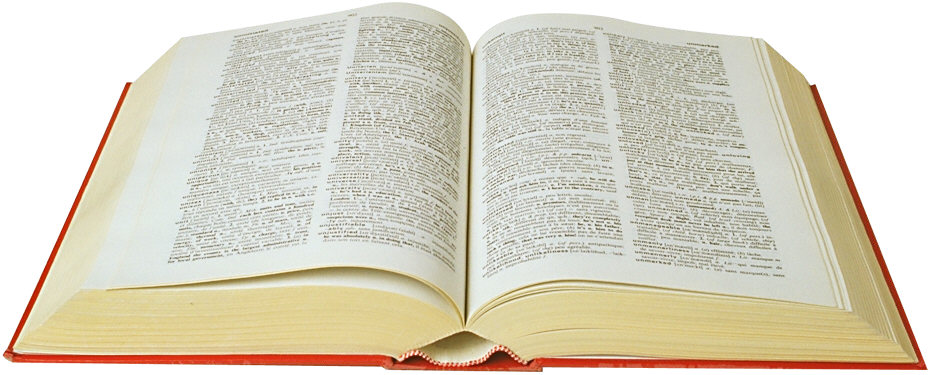
\includegraphics{book}
                    \par
                    %{\small Fonte: Produção do próprio autor.}
                    \fonte{Produção do próprio autor.}
                \end{figure}
                
    
        \section {Equações}
        
        Fórmulas e Equações devem ser destacadas no texto de modo a facilitar sua leitura, sendo numeradas consecutivamente com algarismos arábicos entre parênteses. Fórmulas simples podem aparecer no próprio texto, sem necessidade de numeração.
        
        A equação \ref{eq:integral} de uma equação matemática destacada do texto. É de suma importância indicar o uso do ambiente \verb|equation|, que oferece uma melhor compatibilidade, maior flexibilidade além de referências cruzadas. O ambiente matemático indicado pelos símbolos "\$\$" deve ser evitado para qualquer expressão matemática destacada, sendo utilizado somente em uma expressão matemática simples que aparece junto ao texto.
        
        \begin{equation}
            \label{eq:integral}
            \int\limits_a^b f(x) dx = \lim_{n \to \infty} \displaystyle\sum_{i=1}^{n} f(x_i) \Delta i
        \end{equation}
        %fórmula trocada: \lim_{x \to \infty} PARA  \lim_{n \to \infty} 
        
        
        Uma expressão matemática simples pode ser incluída no corpo do texto. Por exemplo, o triângulo $a^2 = b^2 + c^2$ pode ser escrito utilizando o símbolo "\$" sem problemas. Qualquer expressão matemática pode ser incluída no corpo do texto para elaboração de um raciocínio. Mas toda expressão que se deseja destacar do texto deve ser redigida dentro do ambiente \verb|equation|.
    
        \section{Exemplo de Níveis de Seção}
    
        Agora será ilustrado como se utilizar os diferentes níveis e subníveis de seção em seu documento. Estar atento quanto a identação do código para manter a clareza e organização de seu trabalho.
        
            \section{SEÇÃO EXEMPLO UM}
            Todo título de seção (primeiro nível abaixo do capítulo) deve ser escrita OBRIGATORIAMENTE com letras maiúsculas, dessa forma é garantido que o título de sua seção irá aparecer com letras maiúsculas no Sumário. Todas as demais subseções ou capítulos terão seus títulos formatados automaticamente no Sumário.
            
            %\section{SEÇÃO EXEMPLO DOIS}
            %Novamente, todo título de seção (primeiro nível abaixo do capítulo) deve ser escrita OBRIGATORIAMENTE com letras maiúsculas. Esse padrão deve ser mantido em todo texto.
            
                \subsection{Subseção Exemplo Um}
                \lipsum[8]
                
                \subsection{Subseção Exemplo Dois}
                \lipsum[7]
                
                    \subsubsection{Sub - Subseção Exemplo Um}
                    \lipsum[6]
                    
                    \subsubsection{Sub - Subseção Exemplo Dois}
                    \lipsum[12]
                    
                        \paragraph{Sub - Sub - Subseção Exemplo Um}
                        \lipsum[11]
                        
                        \paragraph{Sub - Sub - Subseção Exemplo Dois}
                        \lipsum[13]

     \chapter{Possíveis Melhorias para o atual Modelo}
        
        Há alguns pontos que poderiam ser incrementados nesse template. Sinta-se à vontade de colaborar com o projeto no repositório do GitHub \footnote{Repositório do modelo de trabalho acadêmico disponível em \url{https://github.com/luisfelipebarbosa/feg-latex.git}} e prover a próxima versão, isto é, a \emph{v1-2}. Os pontos são:
        
        
        \begin{itemize}
            \item prover exemplos genéricos ou reais de como se referencia outros tipos de trabalhos não contemplados nesse template, mas mencionados nas diretrizes;
            \item adicionar imagens vetorizadas de alguns comuns tipos de arquivos, tais como .eps .pdf, o que requer  adicionar  package(s) adicional(s);
            \item adicionar um exemplo de gráfico ilustrativo (formato gif), como mostrado nesse site \footnote{Veja esse exemplo disponível em: \url{https://help.geogebra.org/topic/how-to-include-animated-gif-in-latex-pdf} (acesso em 17 fev. 2019)}. Isto pode ser uma forma bem eficiente de prover resultados de simulações ou fotos sequencias;
            \item por fim, solucionar as open issues explicadas no GitHub.
        \end{itemize}
     
     
     \chapter{Outros Capítulos}
    
        Fique a vontade de estruturar o seu trabalho conforme necessário e de acordo com as recomendações do seu orientador e/ou co-orientador \dots
    
    %------------------------------------------------------------------------------------%
    %                               P Ó S   T E X T U A L                                %
    %                                                                                    %
    % Fim do corpo do texto. A partir desse comando as indicações no sumário serão       %
    % marcadas como 'pós textuais'.                                                      %
    %------------------------------------------------------------------------------------%
    
    \postextual
    
    %------------------------------------------------------------------------------------%
    % R E F E R Ê N C I A S
    %
    % OBRIGATÓRIO. Será gerada automaticamente a partir do arquivo "references.bib".
    %------------------------------------------------------------------------------------%
    
    \bibliography{references}
    
    %------------------------------------------------------------------------------------%
    % A P Ê N D I C E S
    %
    % OPCIONAL. Consiste em um texto ou documento elaborado pelo autor a fim de complementar
    % sua argumentação. Se necessário ter mais de um apêndice, basta adicionar cada um dentro
    % de um dentro de um comando "\chapter". % Se não for utilizar um Apêndice, basta apagar
    % todo o código dessa seção.
    %------------------------------------------------------------------------------------%
    
    \begin{apendicesenv}
        
        \chapter{Título do Apêndice A}
            \lipsum[50]
        
        \chapter{Título do Apêndice B}
            \lipsum[51]
        
    \end{apendicesenv}
    
    %------------------------------------------------------------------------------------%
    % A N E X O S
    %
    % OPCIONAL. Consiste em um texto ou documento não elaborado pelo autor que serve de
    % fundamentação, comprovação ou ilustração ao trabalho. Se necessário ter mais de um
    % anexo, basta adicionar cada um dentro de um dentro de um comando "\chapter".
    % Se não for utilizar nenhum Anexo, basta apagar todo o código dessa seção.
    %------------------------------------------------------------------------------------%
    
    \begin{anexosenv}
    
        \chapter{Título do Anexo A}
            \lipsum[30]
      
        \chapter{Título do Anexo B}
            \lipsum[31]
        
        \chapter{Título do Anexo C}
            \lipsum[32]
      
    \end{anexosenv}
    
\end{document}

